%!TEX root = ../main.tex
%%=====================================================================
%%  §7  NOT REDUNDANT GIVEN A FACTOR MODEL        drafted 2026-08-16
%%
%%  All numbers verified this session (workflow sec7-factor-verify +
%%  ff_lens run; records: _reference/CAPTIONS.md fig_lens_curve entries,
%%  NEWSTATS_hedge_w60.md calendar correction, ff_lens.csv).
%%
%%  SUPERSEDED — do not restore while editing:
%%   - 120-day lens values 0.2878 / 0.1644 / 57.1% / 25.83%  ->
%%     full-sample 0.2776 / 0.1712 / 61.7% / 23.22% (block SEs exist)
%%   - "19/19 unspanned, alpha 6.5-7.7, t 6.9-11.0, R2<=0.003" -> that
%%     was the same-day join on the old 19-arm set; this paper prints
%%     the matched 14 books on each layer's realization calendar
%%   - "no configuration retains less than 40%" -> dead; net of the
%%     matched floor it is 29-51% at m=5. Print the curve instead.
%%   - "the factor model explains almost none of these books" -> dead
%%     (join artifact); correct R2: rules <=0.10, k1 0.12, random 0.22
%%  STILL BINDING:
%%   - be fair to guijarro2025deep: their claim is in passing, under
%%     stated assumptions; we test it, we do not accuse them
%%   - do not conflate this section's "beyond classical factors" with
%%     the GICS-vs-methods comparison elsewhere; separate findings
%%   - GICS must be judged against ITS OWN floor 0.0344, never 0.0614
%%   - m_match is conditional; always pair it with the never-matched %
%%   - the six-named-factor removal ~= THREE PCs, less than five
%%     (0.190 vs 0.193 vs 0.171) — do not flip this comparison
%%   - AR/LM + Monte Carlo size study: prior campaign, different book;
%%     see the TODO below before citing them here
%%=====================================================================
\section{Factors, Peers, and Costs}
\label{sec:factor}

A partition is a special case of a factor model, and clustering-based trading is a special case of peer-based trading. As a factor model, a partition fixes each stock's loading at $1$ on its own group's mean and $0$ on every other group's mean. Latent factor models estimate the loadings freely \citep{fan2013large}. \citet{guijarro2025deep} remark in passing that ``under appropriate assumptions a clustering problem can be solved by a latent factor estimation.'' As a choice of peers, a partition gives every stock in a group the same peer set. The simplest alternative gives each stock its own peer set, the stocks most correlated with it. In this section, we ask whether baselines in either of these more general constructions already contain the information that a partition contributes. We test a partition against factor models in the cross-section and in the time series. In the cross-section, we measure how much of a partition's variance share remains after factors are projected out (\secref{sec:lens}). In the time series, we test whether the portfolios built on the partitions are spanned by the Fama--French five factors plus momentum, by a reversal factor, by the leading principal components, or by the portfolio of the same pipeline run without clustering (\secref{sec:spanning}). To test a partition against per-stock peers, we replace it with per-stock peer regressions and ask the same question of the portfolios (\secref{sec:peer}). Finally, we ask whether the portfolios remain profitable after trading costs (\secref{sec:costs}).

\subsection{Cross-Sectional Projections}
\label{sec:lens}

We ask how much of the cross-sectional variance of a day's market residuals a partition can explain, and how much of that it still explains after the leading principal components are projected out. If a low-dimensional latent factor representation captures the same cross-sectional structure as the partition, projecting out a few leading principal components should substantially reduce the variance share that the partition explains afterward. For each of the $6{,}913$ out-of-sample days, we take the day's cross-section of market residuals (\secref{sec:resid}) and apply the partition's same-day labels. We then record the variance share of \secref{sec:mechanism},
%
\begin{equation}\label{eq:vshare}
  \mathrm{VS}_t \;=\; 1 \;-\; \frac{\overbrace{\textstyle\sum_i s_{it}^2}^{\text{within-group variation}}}{\underbrace{\textstyle\sum_i \bigl(\tilde r_{it} - \bar{\tilde r}_t\bigr)^2}_{\text{total variation}}},
\end{equation}
%
where $\tilde r_{it}$ is the market residual of stock $i$ on day $t$, $s_{it}$ is its group-demeaned residual of \eqnref{eq:relsig}, and $\bar{\tilde r}_t$ is the cross-sectional mean of the market residuals. We use the stocks whose market residuals are complete over the loading window, the trailing $252$ days on which the principal components are estimated.\footnote{This leaves $322$ stocks a day for \textsc{gics} and $479$ to $500$ for the other 11 clusterizers. These stocks are not the same set as the $494$ stocks a day that the fixed trading rule trades in \secref{sec:mechanism}, so the variance shares reported there differ slightly from those here.} Next, we project out common factors. Let $B_t$ be the $\N_t \times m$ matrix of the stocks' loadings on $m$ factors. The projection replaces the vector of market residuals $\tilde r_t$ with
%
\begin{equation}\label{eq:proj}
  \tilde r_t^{\perp} \;=\; \tilde r_t \;-\; \underbrace{B_t \bigl(B_t^{\top} B_t\bigr)^{-1} B_t^{\top}\, \tilde r_t}_{\text{fitted by the factors}} .
\end{equation}
%
We write $\mathrm{VS}_t^{\perp}$ for \eqnref{eq:vshare} computed on $\tilde r_t^{\perp}$ with the same groups. For the principal components, $B_t$ holds the loadings on the leading $m$ principal components, estimated over the loading window and strictly before the day.

Projecting out the five leading principal components removes $39\%$ to $56\%$ of a real partition's variance share (\figref{fig:lens_curve}a). For example, with its singleton groups counted (\appref{app:lensrobust}), the $k$-means-on-residuals partition explains $26.5\%$ of the cross-sectional variance of the day's market residuals.
After five principal components are projected out, it still explains $16.0\%$ of the remainder. This is $60\%$ of its variance share before the projection. We call this ratio the retention,
%
\begin{equation}\label{eq:retention}
  \mathrm{Ret} \;=\; \frac{\sum_t \mathrm{VS}_t^{\perp}}{\sum_t \mathrm{VS}_t},
\end{equation}
%
where both sums run over the $6{,}913$ days. Across the 12
clusterizers, the retention at five principal components ranges from $44\%$ for
\textsc{gics} to $61\%$ for unsigned spectral clustering. By contrast, the random control's variance share is $6.00\%$ before the projection and $5.99\%$ after. Both values are at the degrees-of-freedom floor $(\K-1)/(\N-1) = 5.97\%$, the variance share that $\K$ random groups remove in expectation from any cross-section.\footnote{This floor is computed on the universe used here. On the traded universe of \secref{sec:mechanism}, the same formula gives the $5.88\%$ reported there.} The $\K=1$ control's variance share is zero by
construction.

We also count the leading principal components needed to match a partition's variance share, up to a maximum of $30$, the value of $\K$ (\figref{fig:match_cost}). For the $k$-means-on-residuals partition, $30$ principal components suffice on $79\%$ of days. On those days, about $17$ leading principal components are needed to match its variance share. On the other $21\%$ of days, even $30$ are not enough. For the other 11 partitions, the mean number of principal components needed is $7$ to $11$. For these partitions, $30$ principal components fall short on $0.2\%$ to $3.0\%$ of days. The block-bootstrap standard errors of the variance shares in this subsection are $0.1$ to $0.5$ percentage points, so we omit them from the figures.

The Fama--French factors absorb less than the five leading principal components. We repeat the measurement with the stocks' loadings on nested Fama--French sets (CAPM, then three, five, and six factors) as the columns of $B_t$ in \eqnref{eq:proj}. We estimate these loadings over the same loading window. After the full six-factor set is projected out, the 12 clusterizers keep
$50\%$ to $68\%$ of their variance shares before the projection
(\figref{fig:lens_curve}b). Every real partition's variance share declines gently and stays well above
the degrees-of-freedom floor. For example, the variance share of the $k$-means-on-residuals partition falls from $24.6\%$ after the CAPM projection to $20.6\%$ after three factors, $18.5\%$ after five factors, and $17.8\%$ after six factors. For $k$-means on residuals, the whole six-factor set removes about as much as three principal components and less than five. For all 12 clusterizers, the six factors remove less than five principal components. The random control keeps $99.9\%$ or more of its variance share under each of the seven projections. Its variance share equals the floor, which no projection can remove, so full retention is the expected result.

Loadings conditioned on characteristics absorb the least. We use the four
characteristics available on this panel: size, momentum, short-term
reversal, and realized volatility. Size is the log of market capitalization at the close of day $t$. Momentum is the return from day $t-252$ to day $t-21$, and short-term reversal is the return over the $21$ days ending on day $t$. Realized volatility is the standard deviation of raw returns over the $60$ days ending on day $t$. We standardize each characteristic across the day's cross-section and set a missing value to zero after standardization. When the columns of $B_t$ in \eqnref{eq:proj} are the four standardized characteristics, every real partition keeps
$77\%$ to $85\%$ of its variance share, more than it keeps after three principal
components are projected out. The principal components are estimated strictly before the day, but size, reversal, and volatility are measured through day $t$ itself and so contain that day's own return. Projecting out characteristics that contain the day's own return can remove more of the cross-sectional variance of the day's market residuals than projecting out characteristics measured before the day. The retention of $77\%$ to $85\%$ is therefore, if anything, too low. No factor model whose loadings are linear in these four characteristics can absorb more than this projection does, whatever its coefficients. The bound covers instrumented principal component analysis (IPCA) \citep{kelly2019characteristics}. On their own, the four characteristics explain $13\%$ of the cross-sectional variance of the day's market residuals. The random control's variance share again stays at its degrees-of-freedom floor. Accounting characteristics are not available on this panel, so the bound applies only to these four characteristics.

Under every projection, every real partition keeps a variance share above the degrees-of-freedom floor for its own numbers of groups and stocks. Net of that floor, the retention at five principal components ranges from $28\%$ to $49\%$ across the 12 clusterizers (\appref{app:lensrobust}).

\begin{figure}[tb]
\centering
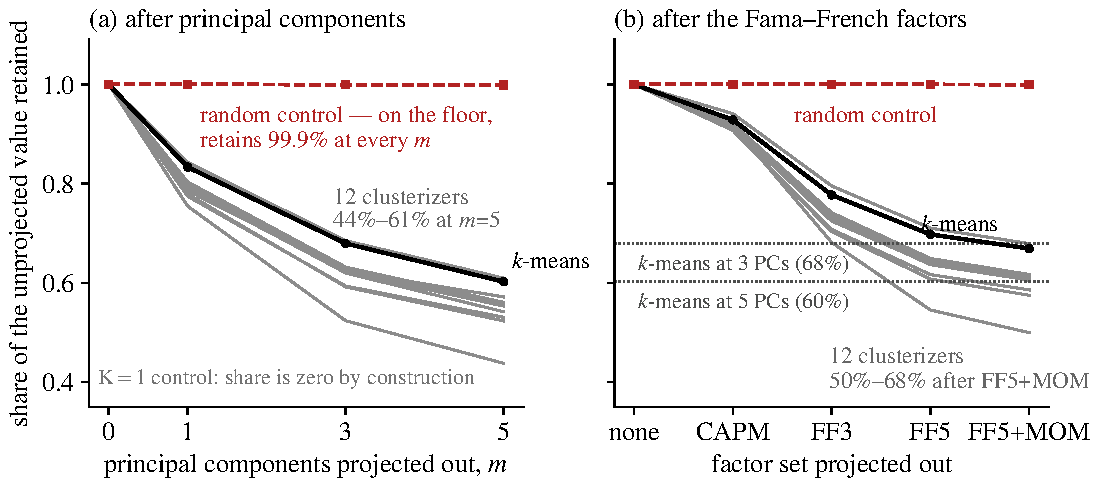
\includegraphics[width=\linewidth]{fig_lens_curve}
\caption{Variance share retained after projecting out principal components and after
projecting out Fama--French loadings. This figure plots each partition's retention (\eqnref{eq:retention}) over the $6{,}913$-day sample. The two panels share a
vertical axis, so the two projections can be compared directly.
(a) The leading principal components, with the first one, the first three, and the first five projected out. (b) The stocks' loadings on nested Fama--French sets, estimated
over the same $252$-day loading window as the principal components and on the aligned
calendar (\appref{app:calendar}). In panel (b), two dotted horizontal lines mark the retention of $k$-means on residuals in panel (a) at three and at five principal components. In both panels,
$k$-means on residuals is black and the other 11 clusterizers are gray. The dashed
red line is the random control, whose variance share is at the degrees-of-freedom floor $(\K-1)/(\N-1)$ and whose
retention is $99.9\%$ or more at every projection, because no projection can remove the floor. The $\K=1$
control's variance share is zero by construction.}
\label{fig:lens_curve}
\end{figure}

\begin{figure}[tb]
\centering
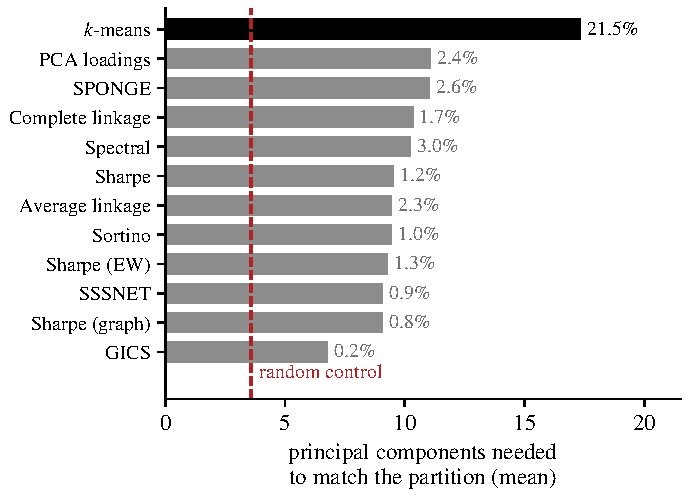
\includegraphics[width=.72\linewidth]{fig_match_cost}
\caption{Principal components needed to match a partition. This figure plots,
for each clusterizer, the mean number of leading principal components needed
to match its partition's variance share, over the
$6{,}913$-day sample. The search stops at $30$ principal components. The mean is taken
over the days on which $30$ suffice, and the percentage beside each bar is the
share of days on which they do not. The bar for $k$-means on residuals is black, and the bars for the other
11 clusterizers are gray. The dashed red line marks the random control.}
\label{fig:match_cost}
\end{figure}


\subsection{Portfolio Spanning Tests}
\label{sec:spanning}

In the time series, we test whether the standard factors span the portfolios' returns, that is, whether each portfolio's alpha against those factors is zero \citep{barillas2017alpha}. Under both trading models, we regress every portfolio's return on the Fama--French five factors \citep{fama2015five} plus momentum \citep{carhart1997persistence} (\tabref{tab:spanning}). For portfolio $p$, the regression is
%
\begin{equation}\label{eq:span}
  \pi_{pt} \;=\; \alpha_p \;+\; \underbrace{\beta_p^{\top} f_t}_{\text{factor exposure}} \;+\; u_{pt},
\end{equation}
%
where $\pi_{pt}$ is the portfolio return of \eqnref{eq:payoff} and $f_t$ is the vector of factor returns on the day on which the portfolio return is realized (\appref{app:calendar}). The later regressions in this section keep this form and change only the regressors in $f_t$. We find that no portfolio is spanned. Every alpha is positive, with $t$-statistics between $4.1$ and $10.7$. The factors explain little of the variation in any of these portfolio returns, with an $R^2$ of at most $0.21$ for the 12 clusterizers. The alphas of \secref{sec:hedge} are therefore not compensation for exposure to these factors.

These rejections are not artifacts of the finite-sample size of the $t$-tests. In a Monte Carlo calibrated to each portfolio's own tails and serial dependence, the empirical size of these tests is $6.6\%$ at a nominal $5\%$ level. Even for the worst-behaved portfolio, the corrected critical value is $2.2$ in $t$ units, which is well below the smallest $t$-statistic of $4.1$ (\appref{app:size}).

The fixed trading rule is a five-day reversal strategy, so the natural factor to add is a reversal factor. The short-term reversal factor of the French library is the closest traded factor, although it is formed on the return over the prior 20 trading days, against five days for the fixed trading rule. We add it to FF5+MOM in the lower block of \tabref{tab:spanning}. Under the fixed trading rule, the reversal factor explains $20\%$ to $25\%$ of the clusterizers' alphas and $38\%$ to $42\%$ of the controls' alphas (\figref{fig:reversal}). For example, the $\K=1$ control's alpha falls from $3.63\%$ to $2.11\%$. Every clusterizer's alpha remains at $3.09\%$ or more (\figref{fig:reversal} shows every value, and \tabref{tab:spanning} reports the ranges). The clusterizers' alpha advantage over the $\K=1$ control therefore widens from $+15.6\%$ to $+54.5\%$. Over the random control, it widens from $+13.1\%$ to $+42.8\%$. However, under the neural trading head, every portfolio loads on the reversal factor at $0.05$ to $0.07$, so the alphas fall by $8\%$ to $13\%$. The alpha advantage barely changes. All 28 portfolios remain unspanned.

The reversal factor is formed by sorting all stocks on their returns over the prior 20 trading days, so it captures reversal relative to the whole market. Demeaning within a real group removes this market-wide part of reversal from the signal and keeps the part that is relative to the group. As a result, under the fixed trading rule, the reversal factor explains more of the controls' alphas than of the clusterizers' alphas. This split of reversal into a market-wide part and a group-relative part follows the inter- and intra-industry decomposition of \citet{hameed2015industries} in spanning form. We use a statistical partition in place of industries and add the two controls, which the industry studies do not have. All portfolios of the neural trading head load lightly on the reversal factor, so they earn little of the reversal premium that the controls earn under the fixed trading rule. Because of this difference in exposure to the reversal factor, the alpha advantage under the fixed trading rule now exceeds that under the neural trading head. In \secref{sec:hedge}, the ordering was the reverse.

\begin{figure}[tb]
\centering
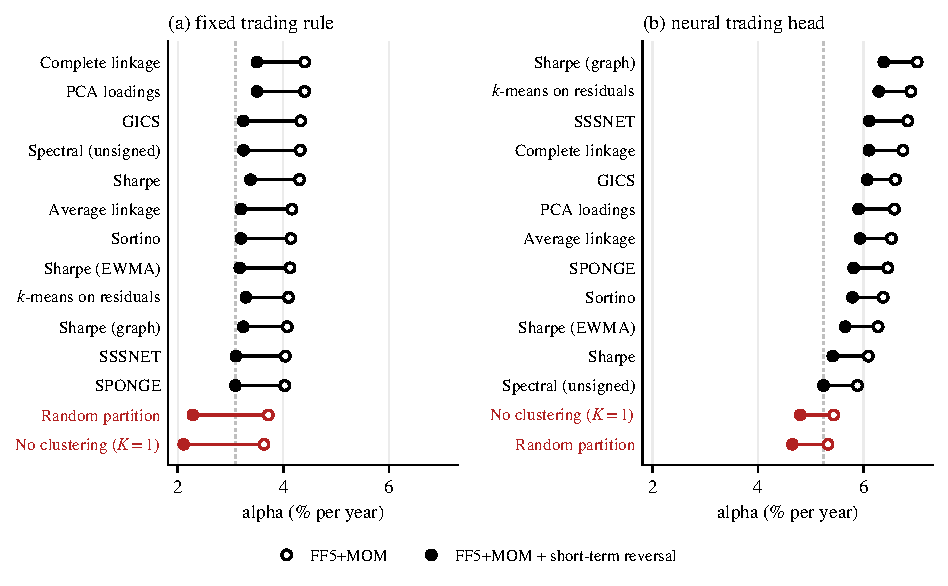
\includegraphics[width=\linewidth]{fig_reversal}
\caption{Alpha before and after the short-term reversal factor. This figure
plots, for each portfolio, its alpha on FF5+MOM (open circle) and its alpha once the
short-term reversal factor is added (filled circle), on the $6{,}913$-day
sample, from the regressions of \tabref{tab:spanning}. (a) The fixed trading rule; (b) the neural trading head. Within each panel, the portfolios are ordered by their FF5+MOM alpha. The two controls are red. The dotted vertical line marks
the lowest alpha with the reversal factor among the 12 clusterizers. Both trading models have gross exposure one, so the two panels share a horizontal axis.}
\label{fig:reversal}
\end{figure}

Although the five leading principal components absorb $39\%$ to $56\%$ of a partition's variance share (\secref{sec:lens}), they absorb almost none of the alpha of its portfolio. When we add the five leading principal components as daily factors, estimated over the same $252$-day loading window as in \secref{sec:lens}, every alpha in \tabref{tab:spanning} changes by at most $0.08$ percentage points, and every $R^2$ changes by at most $0.02$.\footnote{Each principal component's daily return is computed on the market residuals. It is the return of a portfolio with gross exposure one whose weights are the component's loading vector from the loading window. We align the sign of the loading vector from day to day. The five principal-component factors have annualized volatilities from $13.5\%$ down to $5.6\%$. Their premia are not statistically significant.}

The benchmark closest in construction to a clusterizer's portfolio is the portfolio of the same pipeline run without clustering. The $\K=1$ configuration of the same trading model shares the universe and the signal window with a clusterizer's configuration and differs from it only in the partition. To measure directly how much alpha a real partition adds, we therefore regress each clusterizer's portfolio and the random control's portfolio on the $\K=1$ portfolio (\tabref{tab:k1span}). Every clusterizer keeps alpha against the $\K=1$ portfolio. These alphas are $2.24\%$ to $2.86\%$ a year under the fixed trading rule and $2.39\%$ to $4.70\%$ under the neural trading head. Each of these alphas has a $t$-statistic of at least $5.8$. The clusterizers' portfolios load on the $\K=1$ portfolio at $0.37$ to $0.65$. Adding FF5+MOM to these regressions changes the alphas little. Against the $\K=1$ portfolio, each clusterizer keeps $52\%$ to $68\%$ of its FF5+MOM alpha (\tabref{tab:spanning}) under the fixed trading rule and $41\%$ to $68\%$ under the neural trading head. This remaining alpha comes from relative value within the group.

In contrast, the random control keeps little alpha. Under the fixed trading rule, its portfolio loads on the $\K=1$ portfolio at $0.93$, with an $R^2$ of $0.97$. Its alpha is $0.34\%$ ($t = 2.3$). Under the neural trading head, the random control's portfolio loads on the $\K=1$ portfolio at $0.90$, with an $R^2$ of $0.92$. Its alpha is $0.40\%$ ($t = 1.7$).




Under FF5+MOM, the factor loadings also distinguish the controls from the clusterizers. Under the neural trading head, the market loading is $0.105$ for the $\K=1$ control's portfolio and $0.093$ for the random control's portfolio. By comparison, the 12 clusterizers' portfolios load on the market at $0.051$ to $0.077$. Under the neural trading head, a real partition therefore leaves the portfolio with less factor exposure than no partition or a random partition does. This result is consistent with the lower volatility of the clusterizers' portfolios (\secref{sec:hedge}). Under the fixed trading rule, where each portfolio is dollar-neutral by construction, the factors explain little of any portfolio, with an $R^2$ of $0.05$ to $0.07$. The gap in market loading between the controls and the clusterizers is also smaller than under the neural trading head. The market loading is $0.023$ to $0.029$ for the clusterizers, $0.036$ for the $\K=1$ control, and $0.035$ for the random control.

The clusterizers' advantage over the controls holds after 2009 as well as before. When we split the sample at January 2009 (\tabref{tab:era}), alphas fall everywhere in the later subperiod, from $6\%$--$12\%$ to below $4\%$ a year. The clusterizers nevertheless remain separated from the controls in portfolio volatility, in the ordering of the alpha $t$-statistics, and, under the neural trading head, in the alpha advantage over the $\K=1$ control. First, in both subperiods and in both trading models, the controls' portfolios are more volatile than every clusterizer's portfolio. Second, although every alpha $t$-statistic falls, every clusterizer's $t$-statistic still exceeds those of both controls. Over $2009$--$2024$, the lowest clusterizer $t$-statistic under the neural trading head, $2.6$, narrowly exceeds the highest control $t$-statistic, $2.5$. Under the fixed trading rule over the same years, the lowest clusterizer $t$-statistic, $2.8$, exceeds the highest control $t$-statistic, $2.1$. Third, under the neural trading head, the alpha advantage over the $\K=1$ control is larger in the later subperiod, $+29.3\%$ over $2009$--$2024$ against $+20.2\%$ before. In the earlier subperiod, all 12 clusterizers earn more alpha than the $\K=1$ control. In the later subperiod, 11 of the 12 do so. The exception is unsigned spectral clustering.

After 2009, the ordering of the $t$-statistics also holds when we add the reversal factor. Specifically, under the fixed trading rule, the controls' alphas are then no longer significant ($t = 1.5$ for the $\K=1$ control and $1.7$ for the random control). By contrast, every clusterizer's alpha remains significant ($t$ from $2.6$ to $3.6$). Under the neural trading head, the controls keep their alphas in the post-2009 regressions with the reversal factor ($t = 2.1$ for the $\K=1$ control and $2.2$ for the random control). Every clusterizer's alpha has a higher $t$-statistic, from $2.3$ to $5.3$, although the lowest of them exceeds those of the controls by a small margin.

\begin{table}[tb]
\centering
\caption{Spanning against FF5+MOM, with and without a short-term reversal factor, within each trading model}
\label{tab:spanning}
\begin{threeparttable}
\footnotesize
\setlength{\tabcolsep}{2.5pt}
\begin{tabular}{@{}lcccccccc@{}}
\toprule
& \multicolumn{4}{c}{Fixed rule} &
  \multicolumn{4}{c}{Neural head} \\
\cmidrule(lr){2-5}\cmidrule(lr){6-9}
& $\alpha$ & $t_\alpha$ & $R^2$ & $\beta_{\mathrm{Rev}}$
& $\alpha$ & $t_\alpha$ & $R^2$ & $\beta_{\mathrm{Rev}}$ \\
\midrule
\multicolumn{9}{@{}l}{\emph{FF5+MOM}}\\
12 clusterizers & $4.03$--$4.40$ & $6.4$--$7.6$ & $0.05$--$0.07$ & --- & $5.89$--$7.02$ & $8.2$--$10.7$ & $0.14$--$0.21$ & --- \\
$\K=1$ & $3.63$ & $4.1$ & $0.05$ & --- & $5.44$ & $6.8$ & $0.24$ & --- \\
Random & $3.72$ & $4.4$ & $0.05$ & --- & $5.33$ & $7.1$ & $0.22$ & --- \\
\addlinespace
\multicolumn{9}{@{}l}{\emph{FF5+MOM+Reversal}}\\
12 clusterizers & $3.09$--$3.50$ & $5.3$--$6.6$ & $0.27$--$0.31$ & $0.08$--$0.11$ & $5.24$--$6.38$ & $7.5$--$10.4$ & $0.21$--$0.30$ & $0.05$--$0.07$ \\
$\K=1$ & $2.11$ & $2.5$ & $0.25$ & $0.15$ & $4.80$ & $6.1$ & $0.28$ & $0.06$ \\
Random & $2.29$ & $2.8$ & $0.25$ & $0.14$ & $4.65$ & $6.3$ & $0.27$ & $0.07$ \\
\bottomrule
\end{tabular}
\begin{tablenotes}[flushleft]\small
\item \emph{Notes.} This table reports spanning regressions of each portfolio's return on the six factors, and on the six factors plus a short-term reversal factor, under each trading model. The portfolios are those of the 12 clusterizers and the two controls at the common 60-day estimation window, on the $6{,}913$-day sample of \secref{sec:panel} (July 1997 to December 2024). Alphas are in percent a year. FF5+MOM is the Fama--French five factors plus momentum. Reversal is the daily short-term reversal factor (ST\_Rev) of the Ken French data library (CRSP vintage 202606): the average return of the two low-prior-return portfolios minus the average return of the two high-prior-return portfolios from $2 \times 3$ independent sorts on size and prior return, with prior return measured over days $-20$ to $-1$ and the portfolios formed daily. The loading on this factor is $\beta_{\mathrm{Rev}}$. Standard errors are Newey--West($21$) \citep{newey1987simple}. For the neural trading head, the regressions use the seed-averaged return. Each trading model is joined to the factor file on its own realization calendar (\appref{app:calendar}). Both trading models have gross exposure one (\secref{sec:components}).
\end{tablenotes}
\end{threeparttable}
\end{table}

\begin{table}[tb]
\centering
\caption{Spanning against the $\K=1$ portfolio of the same trading model}
\label{tab:k1span}
\begin{threeparttable}
\footnotesize
\setlength{\tabcolsep}{3.5pt}
\begin{tabular}{@{}lcccccc@{}}
\toprule
& \multicolumn{4}{c}{On the $\K=1$ portfolio} & \multicolumn{2}{c}{With FF5+MOM added} \\
\cmidrule(lr){2-5}\cmidrule(lr){6-7}
& $\alpha$ & $t_\alpha$ & $\beta$ & $R^2$ & $\alpha$ & $t_\alpha$ \\
\midrule
\multicolumn{7}{@{}l}{\emph{Fixed trading rule}}\\
12 clusterizers & $2.24$--$2.86$ & $6.9$--$8.2$ & $0.37$--$0.59$ & $0.53$--$0.81$ & $2.19$--$2.84$ & $6.9$--$8.3$ \\
Random & $0.34$ & $2.3$ & $0.93$ & $0.97$ & $0.32$ & $2.1$ \\
\addlinespace
\multicolumn{7}{@{}l}{\emph{Neural trading head}}\\
12 clusterizers & $2.39$--$4.70$ & $5.8$--$9.4$ & $0.42$--$0.65$ & $0.48$--$0.69$ & $2.46$--$4.77$ & $5.8$--$9.5$ \\
Random & $0.40$ & $1.7$ & $0.90$ & $0.92$ & $0.39$ & $1.7$ \\
\bottomrule
\end{tabular}
\begin{tablenotes}[flushleft]\small
\item \emph{Notes.} This table reports regressions of the return of each clusterizer's portfolio and of the random control's portfolio on the $\K=1$ portfolio of the same trading model. The $\K=1$ configuration shares the universe and the signal window with the other configurations of that trading model and differs from them only in the partition. The coefficient $\beta$ is the loading on the $\K=1$ portfolio. Alphas are in percent a year. The last two columns add FF5+MOM to the regressors. Sample, calendar, and conventions are those of \tabref{tab:spanning}, with Newey--West($21$) standard errors and, for the neural trading head, the seed-averaged return. The ranges cover the 12 clusterizers.
\end{tablenotes}
\end{threeparttable}
\end{table}

\begin{table}[tb]
\centering
\caption{Spanning against FF5+MOM by subperiod, 1997--2008 and 2009--2024}
\label{tab:era}
\begin{threeparttable}
\small
\begin{tabular}{@{}lcccccc@{}}
\toprule
& \multicolumn{3}{c}{$1997$--$2008$} & \multicolumn{3}{c}{$2009$--$2024$} \\
\cmidrule(lr){2-4}\cmidrule(lr){5-7}
& $\alpha$ (\%/yr) & $t_\alpha$ & $\sigma$ (\%/yr)
& $\alpha$ (\%/yr) & $t_\alpha$ & $\sigma$ (\%/yr) \\
\midrule
\multicolumn{7}{@{}l}{\emph{Neural trading head}}\\
12 clusterizers & $10.6$--$12.1$ & $9.1$--$10.4$ & $2.6$--$3.2$ & $2.0$--$3.2$ & $2.6$--$5.5$ & $2.7$--$3.6$ \\
$\K=1$ & $9.41$ & $7.0$ & $4.4$ & $2.15$ & $2.3$ & $4.4$ \\
Random & $9.29$ & $7.1$ & $4.2$ & $2.09$ & $2.5$ & $4.1$ \\
\addlinespace
\multicolumn{7}{@{}l}{\emph{Fixed trading rule}}\\
12 clusterizers & $7.1$--$8.1$ & $6.4$--$7.4$ & $2.6$--$3.3$ & $1.7$--$2.2$ & $2.8$--$3.9$ & $2.2$--$3.0$ \\
$\K=1$ & $6.45$ & $4.0$ & $5.2$ & $1.82$ & $1.9$ & $4.2$ \\
Random & $6.52$ & $4.3$ & $4.9$ & $1.89$ & $2.1$ & $4.0$ \\
\bottomrule
\end{tabular}
\begin{tablenotes}[flushleft]\small
\item \emph{Notes.} This table reports the spanning regressions of each portfolio's return on FF5+MOM, split at January $2009$, with the same series and calendars as the FF5+MOM block of \tabref{tab:spanning}, on the $6{,}913$-day sample of \secref{sec:panel}. Here, $\sigma$ is the subperiod's realized annualized volatility of the same series. For the neural trading head, $\sigma$ is therefore that of the seed-averaged return, the convention quoted in the notes to \tabref{tab:moments}. The volatilities in that table are instead computed per head seed and averaged over the five head seeds. 
\end{tablenotes}
\end{threeparttable}
\end{table}

\subsection{Per-Stock Peer Regressions}
\label{sec:peer}

We now turn to per-stock peer sets, from which we build two peer-regression portfolios on this panel. For every stock, we take as its peers the 20 stocks most correlated with it over the trailing $21$-day peer-selection window. We regress the stock's market residual, without an intercept, on the market residuals of its peers over a fit window of $60$ days for one portfolio and $252$ days for the other. The peer-regression residual of stock $i$ on day $t$ is
%
\begin{equation}\label{eq:peerres}
  \varepsilon_{it} \;=\; \tilde r_{it} \;-\; \underbrace{\sum_{j \in P_{it}} \hat b_{ij,t}\, \tilde r_{jt}}_{\text{peer fit}},
\end{equation}
%
where $P_{it}$ is the stock's peer set and $\hat b_{ij,t}$ are the fitted coefficients. The neural trading head takes $\varepsilon_{it}$ as input in place of the group-demeaned residual $s_{it}$. Different stocks' peer sets can overlap. However, no group of stocks shares a common peer set, so the construction does not involve a partition. Each peer-regression portfolio comes from a single run of the trading head at head seed $42$, so no standard deviation across head seeds is available for them. Peer selection is deterministic, so there is no partition seed to redraw either. We therefore do not compare their Sharpe ratios with those of the clusterizers.

In the cross-section, the peer construction absorbs much of a partition's variance share, considerably more than any of the factor projections above.
We repeat the measurement of \secref{sec:lens} after first removing the peer fit, the part of each stock's market residual fitted by its peers over a $60$-day fit window. For 10 of the 12 clusterizers, retention then falls to $25\%$ to $32\%$, against $44\%$ to $61\%$ across all clusterizers under five
principal components. The two exceptions are the $k$-means-on-residuals partition, which retains $52\%$, and \textsc{gics}, which retains $17\%$. The retention of $52\%$ for $k$-means on residuals is inflated by its singletons (\appref{app:lensrobust}). Projecting out the principal components \emph{after} the peer removal changes the retention by at most one percentage point for 10 of the 12 clusterizers and by at most five for the two exceptions. For this measurement, the principal components therefore add almost nothing to what the peer fit absorbs. The random control's variance share remains at its degrees-of-freedom floor through every stage, with a retention of $99.7\%$.

Although the peer fit absorbs much of a partition's variance share in the cross-section, some clusterizers' portfolios keep alpha against the peer-regression portfolios in the time series. We regress the return of every portfolio of the neural trading head on the two peer-regression portfolios,
on FF5+MOM, and on both together (\tabref{tab:peer}). Against FF5+MOM alone, every portfolio keeps its alpha, as in \secref{sec:spanning}. However, against the peer-regression portfolios, the controls and the clusterizers differ. Both controls lose their alpha entirely, with an alpha of $-1.6\%$ a year ($t=-2.2$) for the $\K=1$ portfolio and $-1.4\%$ ($t=-2.0$) for the random control's portfolio. The two peer-regression portfolios therefore explain all of the alpha that this pipeline
earns without a real partition. In contrast, four of the 12 clusterizers keep their alpha, $0.8\%$ to $1.5\%$ a year, with $t$ between $2.1$ and $3.9$. The alphas of the other eight range from $-0.81\%$ to $0.74\%$ ($t$ from $-1.7$ to $1.8$). Unsigned spectral clustering has the lowest of these alphas. Its Sharpe ratio is no higher at $50$ groups than at $10$ (\secref{sec:window}). Among the 12 clusterizers, its portfolio also has the highest volatility (\secref{sec:hedge}) and is furthest below the equal-weight portfolio in Sharpe ratio (\secref{sec:gradient}).

In \eqnref{eq:span}, adding the six factors to the two peer-regression portfolios in $f_t$ raises the alpha of all 12 clusterizers' portfolios by $0.17$ to $0.47$ percentage points. Because the regression has an intercept, the estimated alpha is
%
\begin{equation}\label{eq:alphaid}
  \hat\alpha_p \;=\; \underbrace{\bar\pi_p}_{\text{mean return}} \;-\; \underbrace{\hat\beta_p^{\top} \bar f}_{\text{loadings} \,\times\, \text{mean factor returns}} .
\end{equation}
%
When the factors enter the regression, every clusterizer's portfolio loads less on both peer-regression portfolios. Because the peer-regression portfolios earn positive mean returns, these lower loadings raise $\hat\alpha_p$ in \eqnref{eq:alphaid}. The small positive market loadings of the clusterizers' portfolios offset part of this increase. Adding the reversal factor as well changes the alphas by at most $0.11$ percentage points, because the peer-regression portfolios already absorb the part of the returns that the reversal factor would absorb. The factors raise the alphas and remove common variation from the regression residual. Both effects increase the $t$-statistics. Against the peer-regression portfolios and the factors together, eight of the 12 clusterizers have a $t$-statistic above $1.96$, against four on the peer-regression portfolios alone.

The two controls show that the alpha that the clusterizers keep against the peer-regression portfolios comes from the partition. The controls share the market residuals, the signal window, and the trading head with the clusterizers. They differ from the clusterizers only in the partition, which is absent in the $\K=1$ control and random in the random control. If the shared stages produced the alpha, the controls would also keep a positive alpha against the peer-regression portfolios. Instead, the alphas of both controls are negative, with or without the factors (\tabref{tab:peer}).

Conversely, when we regress each peer-regression portfolio on the equal-weight portfolio of all 12 clusterizers, the alpha is $2.5\%$ a year ($t = 5.5$) for the $60$-day fit and $2.3\%$ ($t = 6.8$) for the $252$-day fit. Although partitions and per-stock peer regressions capture much the same comovement, neither explains all of the other's alpha in our setting. The $R^2$ of a clusterizer's portfolio return on the peer-regression portfolios is positively related to its Sharpe ratio. However, the relation falls just short of significance at the $5\%$ level (\appref{app:peerdist}).

\begin{table}[tb]
\centering
\caption{Spanning against peer-regression portfolios, factors, and both}
\label{tab:peer}
\begin{threeparttable}
\small
\setlength{\tabcolsep}{3pt}
\begin{tabular}{@{}>{\raggedright\arraybackslash}p{3.9cm}cccccc@{}}
\toprule
& \multicolumn{2}{c}{On the peer-regression portfolios}
& \multicolumn{2}{c}{On the six factors}
& \multicolumn{2}{c}{On both} \\
\cmidrule(lr){2-3}\cmidrule(lr){4-5}\cmidrule(lr){6-7}
& $\alpha$ (\%/yr) & $t_\alpha$ & $\alpha$ (\%/yr) & $t_\alpha$ & $\alpha$ (\%/yr) & $t_\alpha$ \\
\midrule
12 clusterizers\tnote{a} & $-0.81$--$1.45$ & $-1.7$--$3.9$ & $5.89$--$7.02$ & $8.2$--$10.7$ & $-0.35$--$1.68$ & $-0.7$--$4.5$ \\
$\K=1$ & $-1.63$ & $-2.2$ & $5.44$ & $6.8$ & $-0.82$ & $-1.2$ \\
Random & $-1.42$ & $-2.0$ & $5.33$ & $7.1$ & $-0.74$ & $-1.1$ \\
\addlinespace
Peer-regression portfolio, $60$-day fit, on the clusterizers' equal-weight portfolio & $2.52$ & $5.5$ & & & & \\
Peer-regression portfolio, $252$-day fit, on the clusterizers' equal-weight portfolio & $2.32$ & $6.8$ & & & & \\
\bottomrule
\end{tabular}
\begin{tablenotes}[flushleft]\footnotesize
\item \emph{Notes.} This table reports, for the neural trading head, spanning regressions of each portfolio's return on the two peer-regression portfolios, on the six factors (the Fama--French five factors plus momentum), and on both. The table also reports the regression of each peer-regression portfolio on the equal-weight portfolio of the 12 clusterizers. In the last two rows, the first pair of columns reports the alpha and $t$-statistic of each peer-regression portfolio on that equal-weight portfolio. Alphas are in percent a year. The six-factor columns repeat the regressions of the neural trading head in the FF5+MOM block of \tabref{tab:spanning} for comparison. The clusterizers' portfolio returns are seed-averaged over the five head seeds, and the peer-regression portfolios come from single runs at head seed $42$. All series are panel-internal, so the regressions share
a common calendar. The factor file is joined at a one-day lag, as for every return series of the neural trading head (\appref{app:calendar}). The $t$-statistics are computed with Newey--West($21$) standard errors.
\item[a] All three ranges cover the 12 clusterizers. On the peer-regression portfolios, four of the 12 keep a $t$-statistic above $1.96$. On the peer-regression portfolios and the six factors together, eight do.
\end{tablenotes}
\end{threeparttable}
\end{table}

%%  §7.3 REWRITTEN 2026-08-21 on v3. Every number recomputed from source
%%  this session: the three spanning specifications from the run logs
%%  with factor_lens.spanning.nw_ols, the retention column from the v3
%%  peer lens (job 61975607, all 6,914 days), the position overlaps from
%%  the verified weight files.
%%  ⛔ HELD BACK, do not add without the runs: (i) any LEVEL comparison
%%     between the peer class and the clusterizers -- the peer arms have
%%     one seed each, so 2.98 against the field's best 2.94 sits inside a
%%     ruler of 0.094 with no dispersion on one side; (ii) the finding
%%     that the peer fit window diversifies where a clusterizer's does
%%     not (peer w60/w252 correlate 0.52 against 0.87-0.89 for pca_load,
%%     agglo_avg and spectral) -- two windows is not a sweep. Both are
%%     requested from the compute branch (seeds on w60/w252, plus w21 and
%%     w120).
%%  ⚠ The peer lens ran with an EMPTY anchor: the v2 npz check was
%%     removed for v3 and the reported "anchor max diff 0.00" is vacuous.
%%     The retention denominators were cross-checked independently here
%%     (unconditional R2 by arm, 300-day sample, agrees within 1 point
%%     and reproduces the ordering); the numerators have no second source.

%%=====================================================================
%%  §6.4  merged from 07_costs.tex on 2026-08-27 (user request)
%%=====================================================================
%%=====================================================================
%%  §8  NOTHING SURVIVES FIVE BASIS POINTS      target 2 pp. NO MORE.
%%
%%  THIS SECTION IS SCOPE, NEVER ARGUMENT. The venue audit calls the
%%  generated draft's six-subsection version "the longest single venue
%%  liability". Two pages, one table, one figure.
%%
%%  ⚠ MANDATORY CAPTION LINE, 2026-08-15 (CORRECTIONS.md N22(h)).
%%    THE COST ROWS ARE NOT AT THE SAME WINDOW AS THE HEADLINE TABLE.
%%    netcost/sbatch_netcost.sh:45-50 routes five arms to their w21
%%    partitions: fv2a, fv3sm, sharpe_fixed and sortino explicitly (their
%%    work.py all read CORR_LOOKBACK = 21), and SPONGE through the
%%    wildcard *) branch to labelcache_sponge_K30_daily_full.pkl, whose
%%    32,423,016-byte signature is the w21 file and not its 32,088,563
%%    w60 twin. SPONGE is the one no reader would suspect, because
%%    nothing in its name or its branch says w21.
%%    ⛔ No netcost/runs/* directory has a MANIFEST, so byte size is the
%%       only in-band proof. Any future netcost pass must write one.
%%
%%    PRINT THIS, FLATLY, AND CLAIM NOTHING BEYOND IT:
%%      "Cost rows are computed at each arm's native clustering window;
%%       for [the five] that is 21 days rather than the 60 used in
%%       Table N."
%%    ⛔ DO NOT add "the difference is unlikely to matter". I asserted
%%       that and it does not survive our own record: N20(e) measures the
%%       traded book as window-INVARIANT for pca_load, agglo_complete and
%%       spectral_unsigned but NOT for agglo_avg (0.158%) or kmeans_ret
%%       (0.615%), driven by singleton frequency, which is itself
%%       window-dependent. Turnover is a function of book size and
%%       membership churn, so window-insensitive turnover is an
%%       assumption the same section contradicts for some arms. Checking
%%       it needs w60 cost runs for those five, which do not exist.
%%
%%  CONTENT:
%%   * 0 of 16 configurations net positive at 5 bps
%%   * turnover 36.5-54.3 %/day, break-even 2.23-3.60 bps
%%   * the structural reason, which connects back to §5: gross return is
%%     6.5-7.7 %/yr against roughly 11.8 %/yr of cost at that level. The
%%     first moment is fixed and modest; turnover exceeds it. This is not
%%     a defect of one implementation
%%   * costs REORDER the field -- the lowest-turnover clustering rises
%%     sharply once costs are charged -- which shows the gross ordering
%%     is not an ordering of economic value
%%   * ⚠ charging five basis points is NOT a monotone transformation of
%%     the gross ranking. Say so; it is the interesting part
%%
%%  COMPARISON TO THE NEAREST PAPER, stated carefully:
%%   brutti2026orthogonal report that clustering REDUCES turnover sharply
%%   in their setup (87.9% to 24.2-24.4%) and do not charge costs at all,
%%   while our configurations show no such gap. Flag the divergence, name
%%   rebalancing frequency as the likely cause, and label it AN OPEN
%%   QUESTION WE HAVE NOT MEASURED. Do not present it as a finding.
%%
%%  LIMITATIONS PARAGRAPH: no market-impact model, no borrow costs, US
%%  large caps only, one residualization scheme, and -- state it here --
%%  K fixed at 30 throughout, with the sweep that would settle whether
%%  the input-parameter result generalizes still unrun.
%%
%%  ⛔ ANY tradability or deployability claim, anywhere in the paper.
%%=====================================================================
\subsection{Transaction Costs}
\label{sec:costs}
The last question is whether the portfolios remain profitable after trading costs.
We measure the daily one-way turnover of a portfolio as $\tfrac{1}{2}\sum_i |w_{it} - w_{i,t-1}|$. Because the gross exposure is one, this turnover is the fraction of the portfolio traded each day. For the 14 portfolios of the neural trading head, it averages $38.2\%$ to $46.9\%$. Turnover varies much less across the 14 portfolios than the gross Sharpe ratio does. The highest turnover is $23\%$ above the lowest, whereas the highest gross Sharpe ratio is $101\%$ above the lowest. The break-even cost is $2.7$ to $3.8$ basis points one-way. At daily rebalancing, every portfolio has a negative net return at five basis points.

At costs below break-even, the net Sharpe ranking follows the gross ranking. At five basis points, it follows turnover. Turnover is not a measure of clustering quality. At one and two basis points, the two controls
remain the two lowest of the 14 portfolios, below each of the 12 clusterizers
in net Sharpe ratio. The rank correlation between the net and the gross ordering is $\rho = 0.98$ at one basis point and $0.91$ at two.

At five basis points, the net ranking largely stops following the gross ranking. The rank correlation with the gross ranking falls to about $0.3$. For example, \textsc{gics} ranks eleventh of the 12 on gross Sharpe ratio but is the least negative portfolio at five basis points. The portfolio of $k$-means on residuals falls from first to seventh of the 14 portfolios. To three decimals, its net Sharpe ratio equals that of unsigned spectral clustering. Both controls move up among the clusterizers. The $\K=1$ control ranks above four of the 12 clusterizers. The random control ranks above one. The \textsc{gics} portfolio rises furthest. This could suggest that a taxonomy has low trading costs, because its labels rarely change. However, the \textsc{gics} portfolio is also the one that depends least on its own labels. On a given day, about $35\%$ of the stocks it trades are not covered by the sector table and are assigned to the group they correlate with most strongly (\tabref{tab:methods}, note e). As a result, the
low turnover of \textsc{gics} cannot be attributed to the taxonomy alone. Average linkage, which does not use a taxonomy, shows the same reordering. Its portfolio turns over $39.7\%$ a day and finishes fourth at five basis points. The gross ranking therefore does not order the portfolios by their value after trading costs. Every comparison in \secsref{sec:riskreturn}{sec:invariance} compares gross performance, before trading costs. Under the fixed trading rule, every clusterizer's portfolio earns a higher gross Sharpe ratio than the portfolio of the $\K=1$ control, $1.46$ to $1.78$ against $0.83$. \citet{brutti2026orthogonal} also find that every clustering-based portfolio earns a higher Sharpe ratio than their no-clustering benchmark. However, our portfolios do not show the turnover reduction that they report. In \appref{app:costs}, we give the cost model, the full table, the same measurement on the fixed trading rule, the comparison with that study, and the limitations of the exercise.
